% Annual Cognitive Science Conference

\documentclass[10pt,letterpaper]{article}

\usepackage{cogsci}
\usepackage{pslatex}
\usepackage{apacite}
\usepackage{graphicx}
\usepackage{amsmath,amssymb}
\usepackage[longnamesfirst]{natbib}
\usepackage{url}

\title{Representing and Learning a Large System of Number Concepts \\ with Latent Predicate Networks}
 
\author{
  {\large \bf Joshua Rule (rule@mit.edu)}\\
  {\large \bf Eyal Dechter (edechter@mit.edu)}\\
  {\large \bf Joshua B. Tenenbaum (jbt@mit.edu)}\\
  MIT, 46-4053, 77 Massachussetts Avenue, Cambridge, MA 02139 USA}

\begin{document}

\maketitle

\begin{abstract}
  The natural numbers are one of the first abstract conceptual systems
  children acquire, forming a foundation on which the rest of
  mathematics and the sciences depend. Psychologists have accordingly
  spent decades investigating number knowledge in children and adults
  as a case study in concept representation and acquisition
  \citep{fuson1988children,galGel2005,Car2009}. Even so, models of
  natural number learning have largely ignored two challenges related
  to the language-like productivity and compositionality of exact
  number concepts: 1) there is an unbounded set of exact number
  concepts, each with distinct semantic content; and 2) people can
  reason flexibly about any of these concepts (even fictitious ones
  like \emph{eighteen-gazillion and thirty-one}). Conventional models
  of concept learning that represent individual concepts as
  collections of prototypes or rules do not naturally explain these
  capacities ({\bf CITATIONS NEEDED}). Models must instead learn the
  structure of the entire infinite set of exact number concepts,
  focusing on how relationships between numbers support reference and
  generalization. Here, we suggest that the latent predicate network
  (LPN) -- a probabilistic context-sensitive grammar formalism --
  facilitates tractable learning and reasoning for exact number
  concepts \citep{DecRulTenming}. We show how the number words and
  their relations to one another can be expressed in this formalism
  and discuss a Bayesian learning algorithm for LPNs, suggesting a
  computational mechanism by which children might learn abstract
  numerical knowledge from linguistic utterances about numbers.

  \textbf{Keywords:}
  child development; concept learning; number; generalization;
  computational model; grammar induction;
\end{abstract}

\section{Introduction}

The natural numbers (1, 2, 3, $\ldots$) are some of the most powerful
concepts yet discovered. They allow precise quantification over finite
sets and thus form a foundation on which nearly all mathematical and
scientific intuition is built. They are among the simplest of
abstract, symbolic structures, yet their usefulness is literally
infinite.

Despite this pivotal role, current evidence suggests humans are
born without an innate understanding of the natural numbers
\citep{Car2009}. Number is instead laboriously acquired over the
course of early childhood, a process stretching well into grade school
\citep{Nat2010}. Even so, the natural numbers are among the first
abstract, symbolic conceptual systems we acquire. Understanding how
number is acquired -- on what basis representation and by what
computational process -- is far more than a simple case study and
promises to significantly increase our understanding of abstraction
and conceptual development.

Natural number acquisition has accordingly been studied intensely and
to great effect. Infant and animal studies suggest several innate
systems, while not containing explicit natural number concepts, are
important for scaffolding our initial representations of number. These
include systems for object individuation and approximate magnitude
\citep{feigenson2004core,dehaene2011number}. One of the most
well-established phenomena of number learning is that the ability to
reliably count sets of objects develops stereotypically, even among
cultures where number is traditionally unimportant
\citep{Wyn1992,JarPianSpelEtAl2014}. Initially, people are
completely unable to associate sets of a given size with the correct
number word. Then, they can do so for sets no larger than one,
followed much later by sets no larger than two, followed again by
sets no larger than three. Typically, children then appear to
generalize the procedure to the other number words they know and can
reliably count out sets of any size, provided they know a sufficiently
large count list. At this point, they are said to have acquired the
\emph{Cardinal Principle} and are variously called \emph{CP-knowers}
or \emph{full counters}.

Attempts to collate decades of number research into a coherent model
have largely focused on the cognitive change that helps children
become \emph{full counters} \citep{Car2009,PianGoodTen2012}. Recent
work suggests, however, that the ability to reliably count sets of
objects, while closely related, is undeniably distinct from our
conceptual knowledge of numbers as representing cardinalities of exact
sets \citep{DavEngBar2012,izard2014toward,JarPianSpelEtAl2014}. More
generally, counting a set of objects requires only a very partial
understanding of number. Models of counting and number learning have
also focused almost exclusively on numbers between one and ten,
presumably because it is during this interval that children become
\emph{full counters}. Most studies, then, examine the development of a
specific skill requiring limited knowledge of a small subset of
numbers.

While the problems of how children link physical sets with the
counting routine and develop a concept of sets as exact collections
are crucial, we direct our attention elsewhere in this paper. We focus
on how children might acquire knowledge of an infinite number system,
particularly for numbers which they are unlikely to ever see counted
out explicitly. We begin by discussing how to represent the sort of
conceptual knowledge needed to describe an infinite number system, and
show how a particular formalism, the Probabilistic Range Concatenation
Grammar (PRCG) can represent number this way
\citep{boullier2005range}. We then show how this grammar can be
learned using Bayesian inference in an LPN, a learning framework for
PRCGs \citep{DecRulTenming}.

\section{Representing Number Knowledge}

To show how a system of concepts like number might be learned, we must
first understand what that system of concepts is and how it might be
represented. We begin by describing several challenges a
representation of number must overcome. We then formally introduce
PRCGs as an answer to these challenges. Finally, we show how this
formalism, initially developed to explain syntactic structures in
natural language, can explain the conceptual structure of number
words.

\subsection{The Challenges of Number}

Relative to many other semantic fields children encounter ({\it e.g.}
the parts of the body, types of furniture in a house), the natural
numbers are highly distinctive.

First, where many semantic fields refer to relatively concrete classes
of objects or object parts, the natural numbers refer primarily to an
abstract property (cardinality) of an abstract entity (sets). Semantic
fields like the parts of the body also tend to be relatively limited
in scope, applying primarily, in this case, to physical parts of
animals. By contrast, natural number is incredibly broad, applying not
only to concrete objects, but also to things like other sets ({\it
  e.g.} three pairs of socks), sounds, events, time periods, people
and other agents, and numbers themselves ({\it e.g.} three threes
makes nine).

% This incredibly broad applicability means that number concepts can often be used, and thus must be understood and represented, without direct perceptual grounding.

Second, there are infinitely many number concepts. Even given a
practically infinite number of instantiated body parts ({\it e.g.}
Timmy's nose), the collection of names for body parts is small ({\it
  e.g.} tail, eye, nose, tummy, ...). By contrast, not only are there
a practically infinite number of natural number instances ({\it e.g.}
three noses), but a truly infinite number of natural number concepts
({\it e.g.} three). Moreover, being infinite, the amount of explicitly
counted, perceptually-grounded evidence children receive relative to
the size of the semantic field is incredibly sparse (When did you last
see exactly 253 objects?) In order to accommodate such an expressive
conceptual system in a finite mind, the concepts themselves must be
constructed as needed in a systematic and compositional manner.
Being infinite and broadly applicable also suggests that numbers can
be learned, represented, and understood without direct perceptual
grounding.

Third, numbers do not uniquely describe cardinalities for children but
initially have distinct meanings related to sequencing, counting,
measuring, ordinality, and several non-numerical meanings ({\it e.g.}
telephone numbers) (Fuson, Richards, Briar, 1982). Even when numbers
do describe cardinalities, interest may not be so much in the
cardinality itself as in some more complex property, such as whether
it is more or less than another cardinality or how it operates
arithmetically via addition, subtraction, multiplication, or division.
Indeed, children may eventually learn about negative and rational
numbers, algebra, geometry, and myriad other mathematical disciplines.
This hugely diverse range of meanings makes it impossible to fully
describe the meaning of \emph{three} without referencing \emph{two},
\emph{four}, and eventually all other numbers. The concept of
\emph{two} (or any other number) is not rightly understood as a single
object, but rather as a web of relationships that hold for some unique
token \emph{two}. The sum collection of these relationships is what
defines the number.

How can we hope to represent a systems of concepts which are: 1)
learnable without direct perceptual grounding; 2) compositionally
constructed; and 3) relationally defined? We propose that the
representation best suited to this sort of structure is a
grammar. Grammars can be induced directly from a stream of utterances,
are highly compositional, and define their constituents based on their
relationships to each other rather than as discrete
objects. Specifically, we propose to use Range Concatenation Grammars (RCGs),
an expressive yet tractable formalism originally developed to model
context-sensitive phenomena in natural language syntax.

\subsection{Probabilistic Range Concatenation Grammars}

RCGs describe precisely those string languages whose parse time is
polynomial in the length of the target
string~\citep{boullier2005range}. An RCG is a 5-tuple $G=(N, T, V, P,
S)$, where $N$ is a finite set of predicate symbols, $T$ is a set of
terminal symbols, $V$ is a set of variable symbols, P is a finite set
of $M \geq 0$ clauses of the form $\psi_0 \rightarrow \psi_1 \dots
\psi_M$, and $S \in N$ is the \emph{axiom}. Each $\psi_m$ is a term of
the form $A(\alpha_1, \dots, \alpha_{\mathcal{A}(A)})$, where $A \in
N$, $\mathcal{A}(A)$ is the arity of $A$, and each $\alpha_i \in (T
\cup V)^*$ is an argument of $\psi_m$. We call the left hand side term
of any clause the \emph{head} of that clause and its predicate symbol
is the \emph{head predicate}.

A string $x$ is in the language defined by an RCG if one can
\emph{derive} $S(x)$. A derivation is a sequence of rewrite steps in
which substrings of the left hand side argument string are bound to
the variables of the head of some clause, thus determining the
arguments in the clause body. If a clause has no body terms, then its
head is derived; otherwise, its head is derived if its body clauses
are derived.\footnote{This description of an RCG language technically
  only holds for \emph{non-combinatory} RCGs, in which the arguments
  of body terms contain only single variables. Since any
  \emph{combinatory} RCG can be converted into a non-combinatory RCG,
  this description suffices.}

PRCGs are RCGs where each clause $C_k \in P$ is annotated with
a probability $p_k$ such that ${\forall A \in N, \,
  \sum_{k:head(C_k)=A} p_k = 1}$. A PRCG defines a distribution over
strings $x$ by sampling from derivations of $S(x)$ according to the
product of probabilities of clauses used in that derivation.\footnote{This is a
well defined distribution as long as no probability mass is placed on
derivations of infinite length; here, we only consider PRCGs with
derivations of finite length.}

\subsection{A Grammar for Number Concepts}

\begin{figure*}[t]
  \begin{centering}
    \includegraphics[width=0.9\linewidth]{grammarOfNumber/gon.pdf}
    \caption{A Range Concatenation Grammar whose strings are valid number words.}
    \label{fig:gon}
  \end{centering}
\end{figure*}

\begin{figure*}[t]
  \begin{centering}
    \includegraphics[width=\linewidth]{parseTrees/parse.pdf}
    \caption{RCG parses for \emph{Number} (Blue), \emph{Successor} (Red), and \emph{More} (Green).}
    \label{fig:parse}
  \end{centering}
\end{figure*}

Having motivated our decision to model concepts as sets of relations
expressed by a grammar, and having described RCGs as our formalism of
choice, we now show that RCGs can capture the conceptual structure of
the natural numbers.

In this initial exploration, we capture three kinds of number
knowledge. First, we show that an RCG can capture the distinction
between valid and invalid number words. While a seemingly basic task,
children struggle to learn that, say, twenty-nine is a number while
twenty-ten is not \citep{FusRicBriar1982}. Second, we capture
predecessor and successor relationships. Unlike the proposed induction
that children make between final number word and final item reached in
a set while counting, we do not attempt to link the physical and
conceptual here. We instead propose a model for an aspect of number
learning that begins earlier and continues later, that of learning the
count list itself. Third, we go beyond mere successor and predecessor
relations to describe more complex aspects of number such as
\emph{More} and \emph{Less}. For any set of $n$ numbers, there are
exactly $n$ valid number words. Because $1$ has no predecessor and we
cannot concisely name the successor of the last number for which we
know the number word ({\it e.g.} What comes after 999,999,999 if we do
not know the word \emph{billion}?), there are actually only $n-1$
valid successor or predecessor relations. There are, however,
$(n^2-n)/2$ more and less relations. Mastering these more abstract
concepts thus requires significantly greater generalization.

Capturing these relations with an RCG is not only possible, but it can
be done quite compactly. Our grammar for the concepts of
\emph{Number}, \emph{Successor}, \emph{Predecessor}, \emph{Less}, and
\emph{More} covers all numbers between 0 and 1 billion, exclusive, and
requires only 216 rules. Even considering just \emph{Number},
\emph{Successor}, and \emph{Predecessor}, these 216 rules cover more
than 500 quadrillion relations. Figure \ref{fig:gon} shows a schematic
of the rules concerned with determining valid and invalid numbers,
while the rest, due to space constraints, can be found
online.\footnote{http://github.com/joshrule/GrammarInduction} This
grammar has not been optimized for compactness or efficiency. A number
of predicates could be compressed or even eliminated, for example, by
implementing \emph{More} with a binary search tree or as the
transitive closure of \emph{Successor}. Instead, we focused on
providing a grammar that would be correct, easy to understand for the
human reader, and fit a prefix-base-suffix understanding of number, as
discussed below.

Intuitively, a number word like \emph{six-hundred thirty-seven} is
valid because we have six units of one hundred each and thirty-seven
remaining units of one each. That is, we have some base unit (hundred)
and we track both how many of them we have (six), and how many of the
next smallest base unit (one) we have (thirty-seven). We denote the
sum of these (six-hundred + thirty-seven) simply by concatenating the
two terms from largest to smallest base (six-hundred thirty-seven).
This structure is recursive. \emph{Nine-thousand seven-hundred
  sixteen} is created by taking nine thousands units and tacking on a
remainder, which is seven hundreds plus its remainder of sixteen ones:
\emph{nine} $\times$ \emph{thousand} $+$ (\emph{seven} $\times$
\emph{hundred} + (\emph{sixteen} $\times$ \emph{one})). Note that
there is no explicit mention of the base \emph{one} in a valid number
word - it is implied and marked by appending $\varnothing$, the empty
string, instead of \emph{one}.

Our grammar similarly uses a prefix-base-suffix system. To conclude
that \emph{six-hundred thirty-seven} is a valid number word (Figure
\ref{fig:parse}), we must show that \emph{six} is a valid prefix for
\emph{hundred} and \emph{thirty-seven} is a valid suffix. We must show
that our use of the largest base is legal, as well as show recursively
that the rest of the number is legal. \emph{Six} is a valid prefix for
\emph{hundred} because it is a number word representing a \emph{ones}
number, a number between one and nine. It would be incorrect for
\emph{hundred} to have no prefix, and it would also be incorrect to
use a prefix larger than \emph{nine}. \emph{Thirty-seven} is a valid
suffix because it is a valid number for a previous base, in this case
$\varnothing$, the ones base. \emph{thirty-seven} is one of these
numbers because it is merely the concatenation of a \emph{decade} word
and a \emph{ones} word. Thus, the compositional use of simple
predicates helps us analyze the structure of a complex phrase like
\emph{six hundred thirty seven} and show that while it is a valid
number word, \emph{hundred six seven thirty} is not. \emph{Successor}
and \emph{More} can similarly be encoded (Figure \ref{fig:parse}),
while \emph{Predecessor} and \emph{Less} can be encoded quite simply
as $\text{Less}(X,Y) \leftarrow \text{More}(Y,X)$ and
$\text{Pred}(X,Y) \leftarrow \text{Succ}(Y,X)$.

These examples help clarify what this grammar represents and how we
accomplish that representation. First, and perhaps most importantly,
\emph{Number} contains no link between set cardinalities and number
words, and \emph{More} lacks a connection to approximate magnitude. We
intend to explore these connections in future work but focus here on
the fact that to know what the number words mean is to know how they
interact with other concepts you already have, including (potentially
innate) pre-existing conceptions of \emph{More} or \emph{Less} used to
differentiate sets, or \emph{Successor} used to memorize songs and
routines. Second, while the conceptual grammar contains a great deal
of knowledge about \emph{fifty-two}, there is no object that in any
sense contains the full meaning of \emph{fifty-two}. The meaning is
simply the collection of relationships which hold for the token
\emph{fifty-two}. Third, the grammar never produces nor parses full
English sentences. This is a grammar for the structure of concepts,
not the structure of language. When attempting to parse something like
\emph{Succ(ninety nine, one hundred)}, we assume some other system
more directly involved in language preprocesses utterances into a
partially predicated state, which is then checked against the
knowledge encoded in our conceptual grammar. Fourth, the names given
to specific predicates have no inherent semantics. \emph{Number} could
just as easily be called \emph{Wug} or \emph{Dax}. What is important
is not a predicate's name, but the relations it enters into with other
predicates and thus the argument strings for which it holds.
Individual words like \emph{hundred} or \emph{nine} also have no
inherent meaning. They acquire meaning through the way each predicate
combines or contrasts them with other words. Finally, we provide a
grammar explaining number relations in terms of English number words,
but that grammar could easily be modified to model different counting
systems, such as those used in French or Mandarin.

\section{Learning Number Knowledge}

How might children learn the knowledge about number that is captured
in the representation presented above? In this section, we present a
computational model of learning over RCGs and take a first step
towards evaluating this model against the learning trajectories and
patterns of error reported in the literature on counting. 

Because the learning problem is computationally challenging and
because much of the focus in the literature on exact number knowledge
has been on counting, we restrict our experiments here to the
successor relation, and, in particular, to learning how to count from
one to a hundred.

Learning to count up to a hundred does not come easily. Studies of
counting in children between three and six years of age, suggests that
although some children are able to count up to a hundred shortly
before entering kindergarten, many have trouble with the task at least
as late as first
grade~\cite{FusRicBriar1982,miller1987counting}. These studies suggest
that children do not learn to count to a hundred by memorizing the
sequence of numbers between on and a hundred. As might be expected of
a system that will eventually be able to count to arbitrarily large
numbers, learning to count to a hundred involves discovering the
pattern that successive number words follow. 

We will model this process of pattern discovery as probabilistic
inference over RCGs and show that some of the interesting phenomena
described in these studies is captured by this model. 

\subsection{Latent Predicate Networks}
Latent Predicate Networks (LPNs) are probabilistic context senstive

\citet{FusRicBriar1982} describe several qualitative phenomena of
count sequence aquisiton and elaboration based on several surveys in
which they asked American children between three and five years of age
to count (either while counting a collection of objects or just
reciting the count world sequence). The learning trajectories and
error patterns they describe have inspired computation modeling
efforts using connectionist networks; for example,
\citet{ma1989modeling} use an associative network to model the errors
that young children typically make when learning the count sequence up
to twenty or thirty. But, to our knowledge, such models have not been
used to study how children acquire the count sequence beyond twenty.

Figure~\ref{fig:fusonTable} shows the highest number correctly reached
by children in various age ranges, as presented in
\citet{FusRicBriar1982}.

\begin{figure}[t]
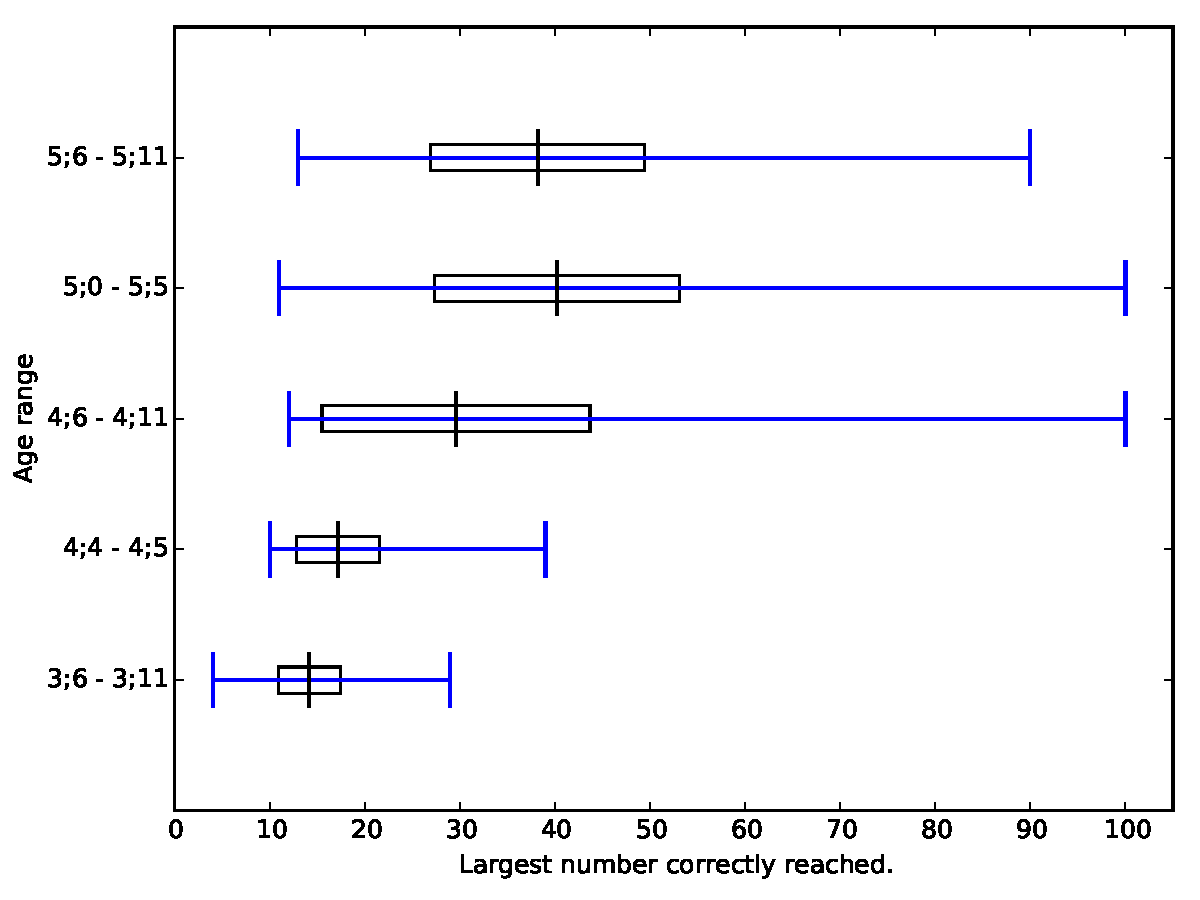
\includegraphics[width=\linewidth]{figures/fuson_table}
\caption{Data from~\citet{FusRicBriar1982} on children's ability to recite the count list. The x-axis shows the highest number correctly reached when children were asked to count starting at ``one.'' Boxes correspond to the standard deviation, central bands to the means, and the whiskers to the range. 
\label{fig:fuson_count_data}}. 
\end{figure}


\begin{figure*}[t]
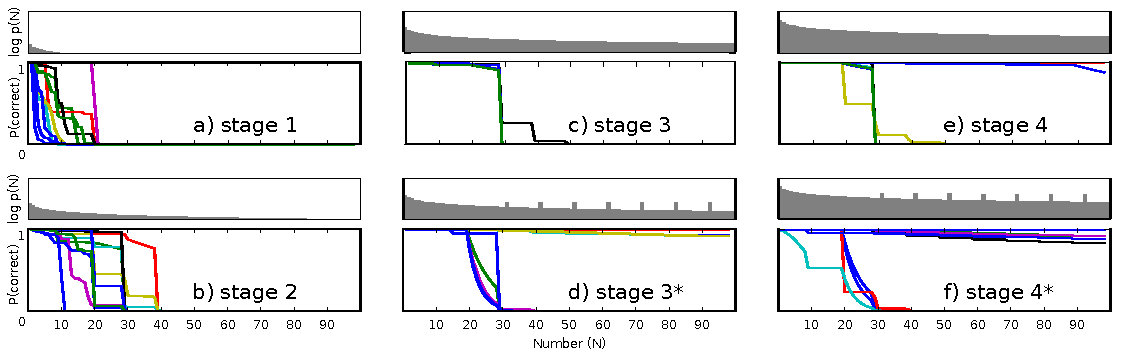
\includegraphics[width=\linewidth]{figures/counting_grid2}
\caption{Our model's performance correctly reciting the count sequence
  having learned with various quantities and types of evidence. Each
  line corresponds to a single run of the learning algorithm given the
  distribution of data shown in the histogram directly above it. For
  each number along the x-axis the y-axis corresponds to the
  probability that model correctly counts from one up to that
  number. The y-axes on the data histograms are shown on a logarthmic
  scale. The simulations in a) were trained on the least data and
  those in b-d) on increasing quantities of data. Those in e) and f)
  were trained on the same data as those in c) and d), respectively,
  with the modification that extra emphasis was placed on the decade
  transitions. \label{fig:counting_grid}}
\end{figure*}

We being by discussing Latent Predicate Networks
(LPNs), our modeling framework.

\subsection{Latent Predicate Networks}


\subsection{}

Eyal

\subsection{Results}

Eyal

\section{Discussion}

%% first half: Eyal

Either way, as these models claim to cover more well-trodden
territory, they should also become correspondingly more quantitative
in their predictions. The ability to generalize as well as the
qualitative similarities we show here between LPNs and children's
overgeneralizations are intriguing, but 

%% second half of discussion

We share a similar vision with the Rational Rules model and descendent
models
\citep{goodman2008rational,T.D.Ullman:2012:1b1b6,PianGoodTen2012} of
exploring concept learning through Bayesian induction of compositional
representations using sparse evidence. We agree that these are
fundamental to understanding concept learning. The major difference is
in how these models represent concepts; both use a grammar, but for
different purposes. Rational Rules models see concepts as specific
sentences in a language defined by a grammar. The (potentially
infinite) hypothesis space over specific concepts is a collection of
logical sentences, or rules, generated by that grammar, and the goal
is to find sentences which apply to collections of objects in the
world. In our model, the hypothesis space is not over sentences in a
grammar but over possible grammars. To wit, the grammars in this paper
are only a few of millions of possible grammars in our hypothesis
space. Moreover, neither these grammars nor sentences in this grammar
represent individual concepts. It is instead the entire language of
the grammar, the network of all possible sentences or relations which,
taken as a whole, describes certain concepts, here \emph{Number},
\emph{Successor}, \emph{Predecessor}, \emph{More}, \emph{Less}, and
supporting predicates like ({\it i.e.} \emph{Decade}, \emph{Prefix},
\ldots). Where Rational Rules models see concepts as specific
sentences in a grammatical language, LPNs see concepts as networks of
grammatically-generated relations.

This comparison holds for the Rational Rules-style model of counting
and CP-acquisition given in \citep{PianGoodTen2012}. This model is
focused on finding a specific sentence which captures the CP, in this
case a program in the simply-typed lambda calculus, rather than on
finding a grammar some of whose relations correctly describe the CP.

More generally, we focus on a different psychological problem than
Piantadosi and colleagues (\citeyear{PianGoodTen2012}) in that we are
not proposing a model of how children acquire their initial number
concepts or the CP. We have no representation of physical sets, and
thus cannot link set manipulation and the counting sequence. Since the
acquisition of \emph{full counting} relies on this link, our current
system is not a model of early number acquisition, nor does it model
the related problem of discovering that sets have exact sizes.
Instead, this paper demonstrates one way that humans might learn
concepts purely from symbolic information provided by utterances.

That said, we see no fundamental incompatibility between the model
presented here and extensions to include approximate magnitude, object
tracking, set manipulation, or more complex morphology ({\it e.g.} the
meaning of \emph{-illion} or \emph{-teen}), as would be needed for a
more comprehensive model of number learning. Far from it, we see our
work here as a first demonstration of LPN's suitability for capturing
a broad range of number concepts, though whether more general models
are best approached by working strictly within the LPN formalism or by
using it as one module within a more complex framework is an open
question. Certainly, the human mind is more powerful than an RCG and
is at least Turing-complete. RCGs provide a tractable way, however, to
explore a restricted subclass of problems. The strategies and
solutions we discover here are also available in Turing-complete
systems, and in fact implemented in one (PRISM Prolog) so our findings
easily generalize to more expressive grammars.

More broadly, we see this paper as growing out of the hypothesis that
much of human learning, including the explosion of knowledge that
occurs during development, can be explained as induction in a formal
language. This vision of the \emph{child-as-hacker} draws on and
extends the notion of the \emph{child-as-scientist}; not only are
children forming theories about the world, but they are simultaneously
developing the very conceptual language they use to formulate those
theories.

% Boullier 2003 shows that RCGs can compute things as sophisticated
% as prime number detection, though by very different means than we
% use here. Even so, understanding how to bring these abilities into a
% symbolic or mixed symbolic/iconic system is an open question.
% similar to Boullier, 2003 in that the interest is in using RCGs to
% capture mathematical concepts. The approach taken here is very
% different though. We're using a fully symbolic, rather than an
% iconic, representation of number. Boullier's work may be
% informative, though for understanding approximate magnitudes and
% other iconic forms of representation.

\section{Acknowledgments}

The authors benefited significantly from conversations with Timothy
O'Donnell and Leon Bergen. This material is based upon work supported
by the Center for Minds, Brains and Machines (CBMM), funded by NSF STC
award CCF-1231216, an NSF Graduate Research Fellowship, and the Eugene
Stark Graduate Fellowship.


\bibliographystyle{apacite}

\setlength{\bibleftmargin}{.125in}
\setlength{\bibindent}{-\bibleftmargin}
\bibliography{cogsci}

\end{document}
